\documentclass{beamer}
\usetheme{CMU}

\usepackage{pgf,pgfarrows,pgfnodes,pgfautomata,pgfheaps,pgfshade}
\usepackage{amsmath,amssymb}
\usepackage[utf8]{inputenc}
\usepackage{colortbl}
\usepackage[english]{babel}
\usepackage{booktabs}
\usepackage{slpython}
\usepackage{underscore}

\author{Luís Pedro Coelho}
\institute{Programming for Scientists}

\graphicspath{{figures/}{figures/generated/}{images/}}

\newcommand*{\code}[1]{\textsl{#1}}


\title{Object Oriented Programming}
\begin{document}

\frame{\maketitle}

\begin{frame}[fragile]
\frametitle{Procedural Programming}
\alert{Procedural programming}: organising programs around functions.

\alert{Object-oriented programming}: organising programs around objects.
\end{frame}

\begin{frame}[fragile] 
\frametitle{Object Oriented Programming}

\begin{block}{OOP}
\begin{description}
\item[Aggregation] organise functions \& data into classes.
\item[Encapsulation] hide information inside methods.
\item[Polymorphism] re-use code for multiple types.
\item[Inheritance] re-use code from one class to build another.
\end{description}
\end{block}
\end{frame}

\begin{frame}[fragile] 
\frametitle{User-Defined Types}

\begin{block}{Built-in Types}
\begin{enumerate}
\item lists
\item dictionaries
\item strings
\item \ldots
\end{enumerate}
\end{block}
\end{frame}

\begin{frame}[fragile] 
\frametitle{Type}
\begin{block}{What's a Type}
\begin{enumerate}
\item A domain of values
\item A set of methods (functions)
\end{enumerate}
\end{block}

\end{frame}

\begin{frame}[fragile] 
\frametitle{Examples of Types}

\begin{block}{List}
\begin{enumerate}
\item Domain: lists
\item Functions: \code{L.append(e),L.insert(idx,e), \ldots}
\item Operators: \code{L[0], 'Rita' in L}
\end{enumerate}
\end{block}

\pause
\begin{block}{Integer}
\begin{enumerate}
\item Domain: $\dots,-2, 1, 0, 1, 2, \dots$
\item Operators: \code{A + B},\ldots
\end{enumerate}
\end{block}
\end{frame}

\begin{frame}[fragile] 
\frametitle{User-defined Types}

Object-oriented programming languages allow us to define new types.

\end{frame}

\begin{frame}[fragile] 
\frametitle{Motivating Example}
\begin{block}{Simple Population Simulation}
\begin{enumerate}
\item We want to simulate a bacterial population.
\item Our environment is a single float $e$.
\item Each bacterium has two characteristics: adaptation $\alpha$ and mutation rate $\sigma$.
\item The smaller the difference $|\alpha-e|$, the better an bacterium is adapted to the world.
\item When an bacterium reproduces, its offspring has adaptation $\alpha + \mathcal{N}(0,\sigma)$
\item At each iteration:
\begin{enumerate}
\item Bacteria die with a probability given by $\lambda\exp(-\lambda|\alpha-e|)$
\item Bacteria that survive, sometimes reproduce.
\end{enumerate}
\end{enumerate}
\end{block}

\end{frame}

\begin{frame}[fragile] 
\frametitle{Bacteria World}
\begin{block}{Bacterium Class}
We define a bacterium class, with two values:
\begin{enumerate}
\item adaptation: its current adaptation value
\item sigma: its variability parameter
\end{enumerate}
and two methods:
\begin{enumerate}
\item \code{P_dead(environ)}: make a stochastic decision on whether the bacteriumdies
\item \code{reproduce()}: make a new bacterium, derived from current one
\end{enumerate}
\end{block}

\end{frame}

\begin{frame}[fragile] 
\frametitle{Using our Bacteria}
\begin{python}
population = [Bacterium(random(),random())
        for i in xrange(nr_inital_bacteria)]
for i in xrange(max_iters):
    bi = 0
    while bi < len(population):
        if population[bi].P_dead(environ) < random():
            del population[bi]
        else:
            bi += 1
    N = len(population)
    for bi in xrange(N):
        if random() < p_reprod:
            population.append(population[bi].reproduce())
    if N >= max_population:
        shuffle(population)
        while len(population) >= max_population:
            population.pop()
\end{python}
\end{frame}

\begin{frame}[fragile] 
\frametitle{Using our Bacteria}

\begin{python}
...
DeltaAdaptation = [math.abs(environ-b.adaptation) 
                    for b in population]
Sigmas = [b.sigma for b in population]
hist(Sigmas)
\end{python}

\end{frame}

\begin{frame}[fragile] 
\frametitle{Classes As Logical Units}
\begin{block}{Class}
A class aggregates data and functions that belong together.
\end{block}
\end{frame}

\begin{frame}[fragile] 
\frametitle{Bacterium Interface}

\begin{block}{Interface}
Functions:
\begin{enumerate}
\item Constructor: Takes the initial adaptation value and sigma.
\item \code{P_dead(environ)}: Probability of dying in this environment.
\item \code{reproduce()}: Return a new Bacterium.
\end{enumerate}
Data elements:
\begin{enumerate}
\item \code{adaptation}: Current adaptation.
\item \code{sigma}: Current sigma.
\end{enumerate}
\end{block}
\end{frame}


\begin{frame}[fragile]
\begin{python}
class Bacterium(object):
    '''
    Bacterium
    ...
    '''
    def __init__(self,adaptation,sigma):
        self.adaptation = adaptation
        self.sigma = sigma
    
    def P_dead(self,environ):
        '''
        prob = bact.P_dead(environ)
        ...
        '''
        return L*math.exp(-abs(self.adaptation-environ)*L)
    def reproduce(self):
        '''...'''
        return Bacterium(self.adaptation +
                             normalvariate(0,self.sigma),
                             self.sigma)
    ...
\end{python}
\end{frame}

\begin{frame}[fragile]
\frametitle{Calling Methods}

\begin{block}{Defining a method}
\begin{python}
class Bacterium(object):
    ...
    def method(self,arg1,arg2):
        '''...'''
        ...
\end{python}
\end{block}

\begin{block}{Calling a Method}
\begin{python}
anim = Bacterium(random(),random())

anim.method(arg1,arg2)
\end{python}
\end{block}
\end{frame}

\begin{frame}[fragile] 
\frametitle{Object Oriented Programming}

\begin{block}{OOP}
\begin{description}
\item[\alert{Aggregation}] organise functions \& data into classes.
\item[\alert{Encapsulation}] hide information inside methods.
\item[Polymorphism] re-use code for multiple types.
\item[Inheritance] re-use code from one class to build another.
\end{description}
\end{block}
\end{frame}

\begin{frame}[fragile]
\frametitle{Simulation of Changing Bacteria}

Why should only adaptation change? Why not \alert{sigma} too?

\end{frame}

\begin{frame}[fragile]
\frametitle{Evolving Bacterium}

\begin{python}
class EvolveSigmaBacterium(object):
    '''...'''
    def __init__(self,adapt,sigma,sigmafact):
        self.adaptation = adapt
        self.sigma = sigma
        self.sigmafact = sigmafact

    def P_dead(self,environ):
        '''...'''
        return L*math.exp(-
                math.abs(self.adaptation-environ)*L)
    
    def reproduce(self):
        '''...'''
        return EvolveBacterium(
            self.adaptation + normalvariate(0,self.sigma),
            self.sigma + normalvariate(0,self.sigma*self.sigmafact),
            self.sigmafact)
\end{python}
\end{frame}

\begin{frame}[fragile]
\begin{python}
population = [EvolveSigmaBacterium(random(),random(),0.5)
        for i in xrange(nr_inital_bacteria)]
for i in xrange(max_iters):
    bi = 0
    while bi < len(population):
        if population[bi].P_dead(environ) < random():
            del population[bi]
        else:
            bi += 1
    N = len(population)
    for bi in xrange(N):
        if random() < p_reprod:
            population.append(population[bi].reproduce())
    if N >= max_population:
        shuffle(population)
        while len(population) >= max_population:
            population.pop()
\end{python}
\end{frame}

\begin{frame}[fragile]
\frametitle{Mixing populations}
We can have a mixed population of $\sigma$-fixed and $\sigma$-changing bacteria!
\end{frame}

\begin{frame}[fragile]
\begin{python}
population = [EvolveSigmaBacterium(random(),random(),0.5)
        for i in xrange(nr_inital_bacteria//2)] + \
        [Bacterium(random(),random())
        for i in xrange(nr_inital_bacteria//2)]

for i in xrange(max_iters):
    bi = 0
    while bi < len(population):
        if population[bi].P_dead(environ) < random():
            del population[bi]
        else:
            bi += 1
    N = len(population)
    for bi in xrange(N):
        if random() < p_reprod:
            population.append(population[bi].reproduce())
    if N >= max_population:
        shuffle(population)
        while len(population) >= max_population:
            population.pop()
\end{python}
\end{frame}


\begin{frame}[fragile] 
\frametitle{Polymorphism}

\begin{block}{Type Polymorphism}
Code is \alert{polymorphic} if it can use different types without change
\end{block}
\end{frame}

\begin{frame}[fragile]
\frametitle{Duck Typing}

\centering
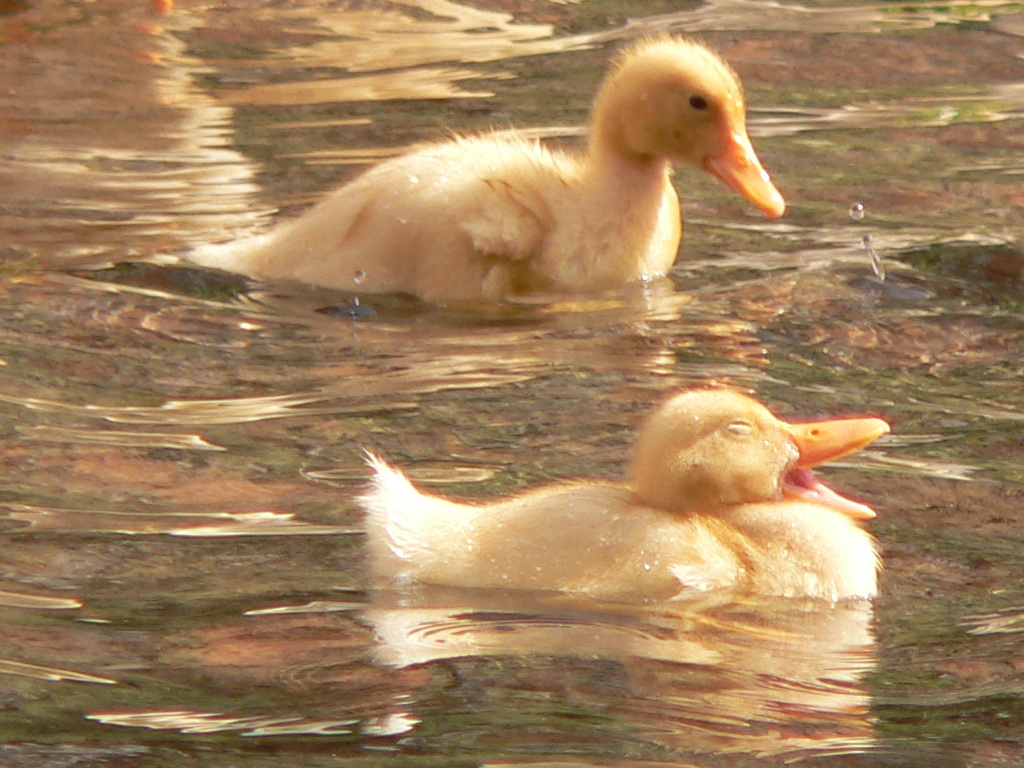
\includegraphics[width=.9\textwidth]{DucksYerevan} % http://upload.wikimedia.org/wikipedia/commons/9/95/Ducks_Yerevan.jpg

\end{frame}



\begin{frame}[fragile] 
\frametitle{Object Oriented Programming}

\begin{block}{OOP}
\begin{description}
\item[\alert{Aggregation}] organise functions \& data into classes.
\item[\alert{Encapsulation}] hide information inside methods.
\item[\alert{Polymorphism}] re-use code for multiple types.
\item[Inheritance] re-use code from one class to build another.
\end{description}
\end{block}
\end{frame}

\begin{frame}[fragile]
\frametitle{Typical Polymorphism}
\begin{block}{Typical examples}
\begin{itemize}
\item Actors in a simulation.
\item File-like objects.
\item Widgets.
\item \ldots
\end{itemize}
\end{block}
\end{frame}

\begin{frame}[fragile]
\frametitle{Inheritance}

The code for EvolveSigmaBacterium is very similar to the code for Bacterium.

\end{frame}

\begin{frame}[fragile]

\begin{python}
class EvolveSigmaBacterium(Bacterium):
    '''
    A type of Bacterium, where $\sigma$ (which controls
    the rate of adaptative mutation) is itself subject
    to mutation (subject to sigma*sigmafact).

    Methods
    -------
        * Constructor:
        * P_dead(environ): inherited from Bacterium
        * reproduce(): 
    '''
    def __init__(self,adaptation,sigma,sigmafact):
        Bacterium.__init__(self,adaptation,sigma)
        self.sigmafact = sigmafact
    def reproduce(self):
        '''...'''
        return EvolveSigmaBacterium(
           self.adaptation + normalvariate(0,self.sigma),
           self.sigma + normalvariate(0,self.sigma*self.sigmafact),
           self.sigmafact)
\end{python}
\end{frame}

\begin{frame}[fragile]
\frametitle{Lyskov Substitution Principle}

If D inherits from C, then\\
you should be able to use D anywhere you previously used C.

\end{frame}

\begin{frame}[fragile]
\frametitle{Behaves-Like}

If D inherits from C, then\\
D should behave-like C.

\end{frame}

\begin{frame}[fragile]
\frametitle{New-Style vs.\ Old-Style Classes}
\begin{python}
class Bacterium(object):
    ...
\end{python}

Are we inheriting from \alert{object}?
\end{frame}


\begin{frame}[fragile] 
\frametitle{Object Oriented Programming}

\begin{block}{OOP}
\begin{description}
\item[\alert{Aggregation}] organise functions \& data into classes.
\item[\alert{Encapsulation}] hide information inside methods.
\item[\alert{Polymorphism}] re-use code for multiple types.
\item[\alert{Inheritance}] re-use code from one class to build another.
\end{description}
\end{block}
\end{frame}

\end{document}
